\documentclass{standalone}
\usepackage{tikz}
\usepackage{textcomp}

\begin{document}

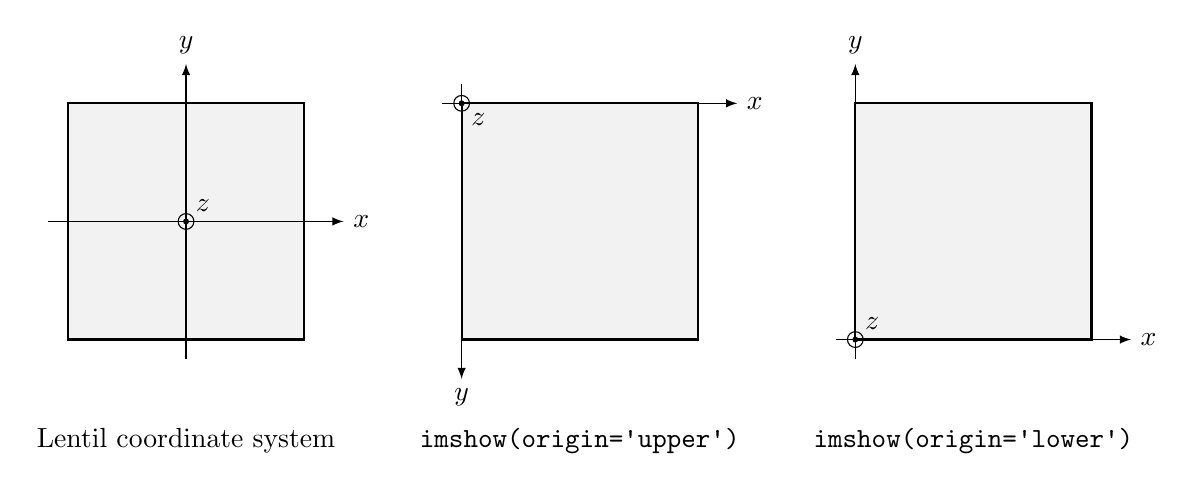
\begin{tikzpicture}

\draw [thick, fill=gray, fill opacity=0.1] (0,0) -- (3,0) -- (3,3) -- (0,3) -- cycle;
\draw[-latex] (-0.25,1.5) -- (3.5,1.5);
\node [right] at (3.5, 1.5) {$x$};
\draw[-latex] (1.5,-0.25) -- (1.5,3.5);
\node [above] at (1.5, 3.5) {$y$};
\draw[fill=black] (1.5,1.5) circle [radius=0.03];
\draw (1.5,1.5) circle [radius=0.1];
\node [above right] at (1.5, 1.5) {$z$};
\node [below] at (1.5,-1) {Lentil coordinate system};

\draw [thick, fill=gray, fill opacity=0.1] (5,0) -- (5,3) -- (8,3) -- (8,0) -- cycle;
\draw[-latex] (4.75,3) -- (8.5,3);
\node [right] at (8.5, 3) {$x$};
\draw[-latex] (5,3.25) -- (5,-0.5);
\node [below] at (5, -0.5) {$y$};
\draw[fill=black] (5,3) circle [radius=0.03];
\draw (5,3) circle [radius=0.1];
\node [below right] at (5, 3) {$z$};
\node [below] at (6.5,-1) {\texttt{imshow(origin=\textquotesingle upper\textquotesingle )}};

\draw [thick, fill=gray, fill opacity=0.1] (10,0) -- (13,0) -- (13,3) -- (10,3) -- cycle;
\draw[-latex] (9.75,0) -- (13.5,0);
\node [right] at (13.5, 0) {$x$};
\draw[-latex] (10,-0.25) -- (10,3.5);
\node [above] at (10, 3.5) {$y$};
\draw[fill=black] (10,0) circle [radius=0.03];
\draw (10,0) circle [radius=0.1];
\node [above right] at (10, 0) {$z$};
\node [below] at (11.5,-1) {\texttt{imshow(origin=\textquotesingle lower\textquotesingle )}};


\end{tikzpicture}
\end{document}
